\documentclass[12pt,a4paper,roman]{article}
\usepackage[utf8]{inputenc}
\usepackage[margin=2.5cm]{geometry}

\title{Research in Data Science and Methodology}
\author{%
\textsc{Enseignant : Oliver Schwander} \\% Your name
\textsc Jean Soler, Nicolas Castanet% Your email address
%\and % Uncomment if 2 authors are required, duplicate these 4 lines if more
%\textsc{Jane Smith}\thanks{Corresponding author} \\[1ex] % Second author's name
%\normalsize University of Utah \\ % Second author's institution
%\normalsize \href{mailto:jane@smith.com}{jane@smith.com} % Second author's email address
}
\date{October 2020}

\usepackage{natbib}
\usepackage{graphicx}
\begin{document}
\maketitle
\begin{abstract}
Ce rapport à pour but d'établir une analyse préliminaire du dataset UC2017 dans le cadre d'un projet pour l'UE d'initiation à la recherche et méthodologie en science des données.
\end{abstract}
\section{Introduction}
Le dataset UC2017 est constitué d'un ensemble de geste réalisés à la mains par plusieurs utilisateurs. Il à pour but l'interaction des hommes avec des robots à travers la reconnaissance de gestes simples par des algorithmes de classifications. 
\newline
Les données propres aux gestes ne sont pas acquis par vidéo mais par des capteurs magnétiques que l'utilisateur porte directement.
Voici les ambitions des ingénieurs pour ce dataset :
\begin{itemize}
    \item Fournir un dataset complet pour l'interaction homme machine.
    \item Avoir de la variance du aux utilisateurs.
    \item Fournir des gestes représentatifs de gestes qui pourraient être exécutés tous les jours et dans n'importe quelles conditions.
\end{itemize}

\section{Dataset UC2017}
Le dataset est constitué de deux types de gestes, les gestes statiques (SG) et les gestes dynamiques (DG). Il compte 24 différents SG et 10 DG.
\newline
\textbf{Voici la campagne de réalisation des gestes}:
\begin{itemize}
    \item SG : 8 utilisateurs, pour un total de 100 répétitions pour les 24 gestes = 24x100 = 2400 exemples.
    \item DG : 6 utilisateurs, pour un total de 131 répétitions pour les 10 gestes = 10x131 = 1310 exemples.
\end{itemize}
Les gestes sont réalisés de la main gauche par des droitiers ce qui induit moins d'assurance dans les gestes. Ceci et la variété des utilisateurs induit de la variance dans les données.

\newpage
On remarque également que chaque utilisateur à réalisé chaque type de geste un nombre identique de fois mais que certains utilisateurs ont réalisé au total beaucoup plus de geste que d'autres. En voici l'illustration sur la répartition des 2400 exemples de SG avec la classe des gestes :

\begin{figure}[h!]
\centering
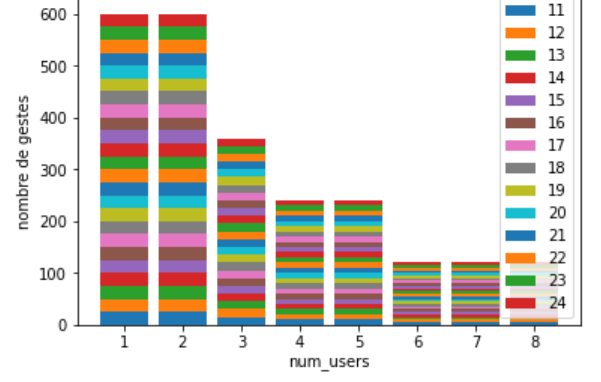
\includegraphics[scale=0.5]{comptage.png}
\caption{nombre de gestes réalisés par chaque utilisateurs, les différentes couleurs correspondants au classes des 24 SG.}
\label{fig:universe}
\end{figure}

Le dataset UC2017 est donc équilibré en classes, avec une variance multi-factorielle (plusieurs utilisateurs, gestes exécutés de manière variables, ordre d'exécution des gestes aléatoire, absence de calibrage, imprécision du placement des capteurs ...). 
\newline

\textbf{Caractéristiques des données :}
Les données sont également biaisées par le manque de proportion des utilisateurs dans la réalisation des gestes : On voit ci-dessus que 1200 gestes sur 2400 ont été réalisés par 2 utilisateurs sur 8. Les algorithmes d'apprentissage seront donc beaucoup pus sensible à une exécution des gestes propre à ces deux utilisateurs (morphologie, habitude de mouvement, etc ...).



Les SG sont représentés par les caractéristiques de la mains à un instant donné tandis que les DG sont représentés par les caractéristiques de la mains au court du temps (le temps de réalisation d'un DG n'est pas fixe).
\newline
Les caractéristiques des gestes sont obtenues à l'aide d'un gant et d'un traceur magnétique. \textbf{Le gant à pour but de capter la forme, la position et l'orientation de la main}. Il possède 22 capteurs situés au niveau des articulations des doigts, du poignet et de la paume, chaque capteurs envoi donc un signal proportionnel à l'angle de l'articulation correspondante $g1, g2, ..., g22$.
\newline
\textbf{Le traceur magnétique de son coté à pour but de mesurer la position et l'orientation du poignet dans l'espace}. Il en résulte 6 nouveaux signaux : $l1, l2, l3$ correspondant à la position dans l'espace et $l4, l5, l6$ correspondants à différentes angles du poignet dans l'espace. 









\bibliographystyle{plain}
\bibliography{references}
\end{document}
